\documentclass[a4paper,11pt]{article}


% \usepackage[francais]{babel}
\usepackage[T1]{fontenc}
\usepackage[utf8]{inputenc}
\usepackage{lmodern}
\usepackage{microtype}
\usepackage{hyperref}
\usepackage{graphicx}
\usepackage{verbatim}
\usepackage{amsmath}
\usepackage{amssymb}
\usepackage{caption}
\usepackage{subcaption}
\usepackage{fullpage}
\usepackage{float}

\DeclareMathOperator*{\argmax}{argmax}
\DeclareMathOperator*{\argmin}{argmin}


\begin{document}
\title{Weibull - Mixed Weibull - Cox Proportional Hazards Model \\ relpy new statistical features}
\author{Ariel Shemtov}
\date{March 2015}
\maketitle


\section{Weibull fitting}

\subsection{PDF}
Weibull PDF $f^W$:

$$ f^{W} (x,\Theta=(\beta,\eta)) =  \frac{\beta}{\eta} \left( \frac{x}{\eta} \right)^{\beta-1} e^{-(\frac{x}{\eta})^{\beta}} $$

\subsection{Likelihood}

\[
L(\Theta) = \sum_{i=1}^f ln\left( \frac{\beta}{\eta} (\frac{x_i}{\eta})^{\beta-1} \right) - \sum_{i=1}^{n} \left( \frac{x_i}{\eta}\right)^{\beta} 
\]
where $f$ is the number of failure points (indeces from 1 to $f$: failures, from $f+1$ to $n$: suspensions).

\subsection{MLE}


Let's take a look at the gradient of the Log-likelihood:


$$
\nabla L(\Theta) =
\begin{cases}
\frac{f}{\beta} + \sum\limits_{i=1}^f \ln\left( \frac{x_i}{\eta} \right) - \sum\limits_{i=1}^n \left(\frac{x_i}{\eta}\right)^{\beta} \ln\left( \frac{x_i}{\eta} \right) \\
-\frac{f\beta}{\eta} + \frac{\beta}{\eta} \sum\limits_{i=1}^{n} \left(\frac{x_i}{\eta}\right)^{\beta}
\end{cases}
= 0
$$

The second equation gives us a relation between $\eta$ and $\beta$:

$$
\eta = \left( \frac{\sum\limits_{i=1}^n x_i^{\beta}}{f} \right)^{1/\beta}
$$

Reinjecting this formula into the likelihood, we get a new objective function 

\begin{align*}
f(\beta) & = L(\beta, \eta(\beta)) \\ \
		 & = fln(\beta)- fln\left( \sum\limits_{i=1}^n x_i^{\beta} \right) + (\beta - 1)\sum_{i=1}^f ln(x_i) + \text{cst}
\end{align*}

Deriving it, we obtain a new equation:

\begin{align*}
\nabla f(\beta) & = \frac{f}{\beta}  - \frac{f \sum\limits_{i=1}^n ln(x_i) x_i^{\beta} }{\sum\limits_{i=1}^n x_i^{\beta}} + \sum_{i=1}^f ln(x_i) \\ \
				& = 0
\end{align*}

$$
\frac{1}{\beta}  - \frac{\sum\limits_{i=1}^n ln(x_i) x_i^{\beta} }{\sum\limits_{i=1}^n x_i^{\beta}} + \frac{1}{f}\sum_{i=1}^f ln(x_i) = 0
$$

Solving it would give us the optimal $\beta$. 

To solve it, we need to apply the Newton descent method on either of these 2 functions: 

$$
f(\beta) = \frac{1}{\beta}  - \frac{\sum\limits_{i=1}^n ln(x_i) x_i^{\beta} }{\sum\limits_{i=1}^n x_i^{\beta}} + \frac{1}{f}\sum_{i=1}^f ln(x_i) 
$$

$$
g(\beta) =   \frac{\sum\limits_{i=1}^n x_i^{\beta}}{\sum\limits_{i=1}^n ln(x_i) x_i^{\beta}} - \frac{\beta}{1+\beta\frac{1}{f}\sum_{i=1}^f ln(x_i)} 
$$

\paragraph{f vs. g}

Let's look at an example plot of f and g:

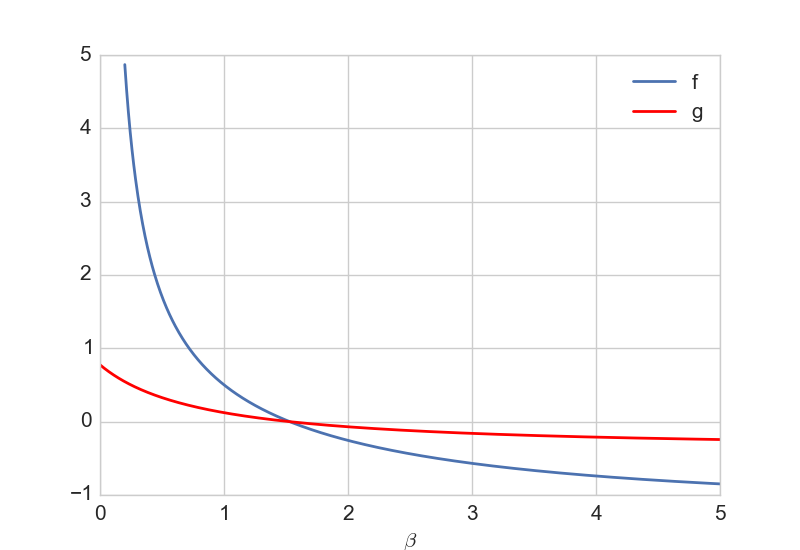
\includegraphics[scale=0.5]{newton_plot2.png}

f goes to infinity in 0, so if close to 0, Newton will be really unefficient. 
Also, complicated to find a reliable starting point.

On the other hand, g is globally way flatter, and 0 is finite, so good match for a starting point.


We apply Newton to g:

$$
g'(\beta) = 1 - \frac{\sum\limits_{i=1}^n ln(x_i)^2 x_i^{\beta}\sum\limits_{i=1}^n x_i^{\beta}}{\left(\sum\limits_{i=1}^n ln(x_i) x_i^{\beta}\right)^2} - \frac{1}{\left( 1 + \frac{\beta}{f}\sum\limits_{i=1}^n ln(x_i)\right)^2}
$$

\section{Mixed Weibull fitting}

\subsection{Mixed Weibull probability distribution}

See: \href{http://reliawiki.org/index.php/The_Mixed_Weibull_Distribution}{The Mixed Weibull Distribution}

Mixed Weibull PDF $f^{MW}$:

$$ f^{MW} (x,\Theta) = 
\sum_{j=i}^{S} \frac{N_j}{N}\frac{\beta_j}{\eta_j} \left( \frac{x}{\eta_j} \right)^{\beta_j-1} e^{-(\frac{x}{\eta_j})^{\beta_j}} $$

where :
\begin{itemize}
	\item $S$ is the number of subpopulationss
	\item $N_i$ is the cardinal of subpopulation number $i$
	\item $N$ is the total size of the sample
	\item $\Theta$ is the set of parameters: $ \left\{ \beta_1, \beta_2, \cdots, \beta_S, \eta_1, \cdots, \eta_S, N_1, \cdots, N_S \right\} $ \\

\end{itemize}

We can see this Mixed Weibull PDF as a sum of Weibull distributions weighted by the shares of each subpopoulation $ \pi_j = \frac{N_j}{N} $, where $\sum \pi_j = 1$.

The PDF becomes:
$$  f^{MW} (x,\Theta) = 
\sum_{j=i}^{S} \pi_j f^W (x,\theta_j) $$

\subsection{Log-likelihood}

Given an input data vector of size $n$ $X = (x_1, \cdots, x_n)$, the likelihood of the Mixed Weibull is:
\begin{align*}
L(\Theta) & = \sum_{i=1}^{n} ln(f^{MW} (x,\Theta)) \\ \
		  & = \sum_{i=1}^{n} ln\left(\sum_{j=i}^{S} \pi_j f^W (x_i,\theta_j)\right) \\ \
		  & = \sum_{i=1}^{n} ln\left(\sum_{j=i}^{S} \pi_j\frac{\beta_j}{\eta_j} \left( \frac{x_i}{\eta_j} \right)^{\beta_j-1} e^{-(\frac{x_i}{\eta_j})^{\beta_j}} \right)
\end{align*}

\subsection{MLE}

The problem becomes: find $\Theta^*$ such that
$$ \Theta^* = \argmax_{\Theta} L(\Theta) = \argmax_{\pi_1,\beta_1,\eta_1,\cdots,\pi_S,\beta_S,\eta_S} \sum_{i=1}^{n} ln\left(\sum_{j=i}^{S} \pi_j\frac{\beta_j}{\eta_j} \left( \frac{x_i}{\eta_j} \right)^{\beta_j-1} e^{-(\frac{x_i}{\eta_j})^{\beta_j}} \right)$$

Under constraint: $\sum_{j=1}^{S} \pi_j = 1$


\subsection{Dealing with supension data}

In case the data shows suspension, we need to tweak the objective function, the same way we would do for a Weibull distribution. 


If we have $f$ failures, $n-f$ suspensions, the log-likelihood becomes:

\begin{align*}
L(\Theta) = \sum_{i=1}^{f} ln\left(\sum_{j=i}^{S} \pi_j\frac{\beta_j}{\eta_j} \left( \frac{x_i}{\eta_j} \right)^{\beta_j-1} e^{-(\frac{x_i}{\eta_j})^{\beta_j}} \right) +
\sum_{i=f+1}^{n} ln\left(\sum_{j=i}^{S} \pi_j e^{-(\frac{x_i}{\eta_j})^{\beta_j}} \right)
\end{align*}


To keep it simple, I'll keep using $f^W$ in the equations, but the form above is the right one to use.

\subsection{Expectation Maximization Algorithm}

We are using the MLE to find the parameters. In order to maximize the Log-Likelihood, we are using the Expectation-Maximization algorithm.

Basically, read wikipedia article: \href{http://en.wikipedia.org/wiki/Expectation%E2%80%93maximization_algorithm}{Expectation Maximization Algorithm}

French article with a nice example: \href{http://fr.wikipedia.org/wiki/Algorithme_esp%C3%A9rance-maximisation#Exemple_d.C3.A9taill.C3.A9_:_application_en_classification_automatique}{Algorithme esperance-maximisation} \\

We define the set of random variables $Z = \{ z_{ij} \in \{0,1\} ,\quad i \in [\![1,n]\!], j \in [\![1,S]\!] \}$ as:
$$ z_{ij} = \begin{cases} 1 & \text{if $x_i$ belongs to population j} \\ 0 & \text{otherwise} \end{cases} $$ 

The Log-likelihood then becomes:

$$ L(\Theta) = \sum_{i=1}^{n} \sum_{j=i}^{S} z_{ij} ln( \pi_j f^W (x_i,\theta_j) )$$

We don't have acess to $z_{ij}$, we can only estimate it with its expectation (expectation step) and then refine this estimation at each iteration.

The problem of finding $\Theta$ comes down to iterating the sequence $\left\{ \Theta^k \right\}$ which converges to $\Theta^*$, the desired set of parameters:
$$ \Theta^{k+1} = \argmax_{\Theta} F(\Theta, \Theta^k) = \sum_{i=1}^{n} \sum_{j=i}^{S} E \left( z_{ij} | x, \Theta^k \right) \ln \left(\pi_j f^W (x_i,\theta_j)\right) $$

The algorithm includes 2 steps at each iteration:
\begin{itemize}
	\item the Expectation (step E): the value of the expectation at iterate k is estimated using Bayes' theorem
	$$ a_{ij}^k =  E \left( z_{ij} | x, \Theta^k \right) = \frac{\pi_j^k f^W (x_i,\theta_j^k)}{\sum_{l=1}^{S} \pi_l^k f^W (x_i,\theta_l^k)} $$
	\item the Maximization (step M): computes $\left\{ \Theta^{k+1} \right\}$ solving the optimization subproblem under constraint $\sum \pi_j = 1$.

	$$ \Theta^{k+1} = \argmax_{\Theta} \left\{ \sum_{i=1}^{n} \sum_{j=i}^{S} a_{ij}^k \ln \left(\pi_j f^W (x_i,\theta_j)\right) \right\}$$
	Thanks to the separability properties\footnote{
			  \textbf{Separability property} in a nutshell:
			  Given a function $f$ of 2 independant sets of variables $X$ and $Y$, if there exist 2 functions $g$ and $h$ such that:
			  $$ f(X,Y) = g(X) + h(Y)$$
			  then:
			  $$ \max_{X,Y} f(X,Y) = \max_X g(X) + \max_Y g(Y) $$	
			 } of the objective function: 

	\begin{align*}
	\max_{\Theta} \left\{ \sum_{i=1}^{n} \sum_{j=i}^{S} a_{ij}^k \ln \left(\pi_j f^W (x_i,\theta_j)\right) \right\}
	& = \max_{\Theta} \left\{ \sum_{j=i}^{S}  \sum_{i=1}^{n} \left( a_{ij}^k \ln \left(\pi_j \right) +  a_{ij}^k \ln \left(f^W (x_i,\theta_j)\right) \right) \right\} \\ \
	& =  \max_{\Pi} \left\{\sum_{j=i}^{S} \sum_{i=1}^{n} a_{ij}^k \ln \left(\pi_j \right) \right\} + \max_{\theta_j} \left\{ \sum_{j=i}^{S}  \sum_{i=1}^{n} a_{ij}^k \ln \left(f^W (x_i,\theta_j)\right) \right\} \\ \
	& =  \max_{\Pi} \left\{\sum_{j=i}^{S} \sum_{i=1}^{n} a_{ij}^k \ln \left(\pi_j \right) \right\} +   \sum_{j=i}^{S} \left\{ \max_{\theta_j} \sum_{i=1}^{n} a_{ij}^k \ln \left(f^W (x_i,\theta_j)\right) \right\}
	\end{align*} 
	where $\Pi$ is the set of parameters $\Pi = \{ \pi_1, \cdots, \pi_S\} $.

	It results in 2 optimization sub(sub)problems: 

	Sspb 1: $$\begin{cases} \max_{\Pi} \sum_i\sum_j a_{ij}^k ln(\pi_j) \\ s.t. \sum_{j} \pi_j = 1 \end{cases} $$
	Sspb 2: $ \forall j$, $$\max_{\theta_j} \sum_{i=1}^{n} a_{ij}^k \ln \left(f^W (x_i,\theta_j)\right) $$

\subsection{First subproblem}

Let's write the Langrangian $l$ of the problem:
$$ l(\Pi,\lambda) = \sum_j \left( ln(\pi_j) \sum_i a_{ij}^k \right)  + \lambda \left( \sum_{j} \pi_j - 1 \right) $$

According to the KKT conditions, the solution couple $(\Pi^*,\lambda^*)$ verifies:
$$ \lambda^* > 0 $$
$$ \nabla l (\Pi^*,\lambda^*) = 0 $$
resulting in :
$$ \begin{pmatrix} \frac{\sum_i a_{i1}^k}{\pi_1^*} - \lambda^* \\ \vdots \\ \frac{\sum_i a_{iS}^k}{\pi_S^*} - \lambda^* \end{pmatrix}  = 0 $$

Finally, we obtain that $\forall j$,
$$ \pi_j^* = \lambda^* \sum_i a_{ij}^k $$
And thanks to the constraint condition:
$$ \lambda^* = \frac{1}{\sum_i\sum_j a_{ij}} = \frac{1}{n} $$

Therefore, $\forall j$, 
$$ \pi_j^{(k+1)*} = \frac{1}{n} \sum_i a_{ij}^k $$

\subsection{Second subproblem}

We can notice that the quantity $ \sum_{i=1}^{n} a_{ij}^k \ln \left(f^W (x_i,\theta_j)\right) $ is almost the same as the the log-likelihood function of the Weibull: $ L(x,\theta) = \sum_{i=1}^{n} \ln \left(f^W (x_i,\theta_j)\right)$ up to a constant multiplier for each term. \\

We can use a slightly modified version of fitWeibull to solve it, using the Newton algorithm. \\

Equation to solve for Weibull:
$$ \frac{1}{\beta} - \frac{\sum_{i=1}^{n} \ln (x_i) x_i^{\beta}}{\sum_{i=1}^{n} x_i^{\beta}} + \frac{\sum_{i=1}^{r} \ln (x_i)}{r} = 0 $$
Equation to solve for Mixed Weibull:
$$\forall j, \quad \frac{1}{\beta} - \frac{\sum_{i=1}^{n} a_{ij} \ln (x_i) x_i^{\beta}}{\sum_{i=1}^{n} a_{ij} x_i^{\beta}} + \frac{\sum_{i=1}^{r} a_{ij} \ln (x_i)}{\sum_{i=1}^{r} a_{ij}} = 0 $$

\end{itemize}

\section{Cox-Proportional Hazards model}

\subsection{Definition of the model}

See: \href{http://reliawiki.com/index.php/Proportional_Hazards_Model}{Relia-Wiki}

The model is defined thanks to the instantaneous failure rate $\lambda$.
Given:
\begin{itemize}
\item a failure time $t$
\item a set of covariates $X = [x_1,\cdots,x_m]$
\item a set of weights $A = [a_1,\cdots,a_m]$
\item a baseline failure rate $\lambda_0$,
\end{itemize}
the instantaneous failure rate in the Cox-Proportional hazard model is defined as:
$$\lambda(t,X) = \frac{f(t,X)}{R(t,X)} = \lambda_0 (t) e^{\sum a_j x_j} $$
where $f$ is the PDF of the distribution and $R$ is the reliability function.

The baseline failure rate $\lambda_0$ determines the underlying distribution that is going to be used.

For the Weibull distribution, it is:
$$\lambda_0 (t) = \frac{\beta}{\eta} \left( \frac{t}{\eta} \right)^{\beta - 1}$$

\subsection{Log-likelihood}

$$ L(\Theta) = \sum_{i=1}^{f} ln(\beta t_i^{\beta-1} e^{\sum\limits_{j=0}^m a_j x_{ij}}) - \sum_{i=1}^{n} t_i^{\beta} e^{\sum\limits_{j=0}^m a_j x_{ij}} $$

Here, we are adding a new constant covariate equal to 1  $x_0 = [x_{10},\cdots,x_{n0}] = [1,\cdots,1]$ to go with a new weight $a_0$ so that we can include $\eta$ in the sum:
$$ a_0 = -\beta ln(\eta)$$

\subsection{MLE}

Solving for $a_0$:
$$ \frac{\partial L}{\partial a_0} = f - e^{a_0} \sum_{i=1}^{n} t_i^{\beta} e^{\sum_{j=1} a_j x_{ij}} = 0 $$

This equation gives us $a_0$ function of the other parameters:
$$a_0 = ln \left( \frac{f}{\sum t_i^{\beta} e^{\sum a_j x_{ij}}} \right)$$

New objective function obtained by reinjecting this expression into the Likelihood:

$$ L(\beta,A) = fln(\beta) +(\beta-1)\sum_{i=1}^{f} ln(t_i) - fln(\sum_{i=1}^n t_i^{\beta} e^{\sum a_j x_{ij}}) + \sum_{i=1}^n \sum_j a_j x_{ij} $$

Gradient:
$$\frac{\partial L}{\partial \beta} = \frac f\beta +\sum_{i=1}^{f} ln(t_i) - \frac{f\sum_{i=1}^n ln(t_i)t_i^{\beta} e^{\sum a_j x_{ij}})}{\sum_{i=1}^n t_i^{\beta} e^{\sum a_j x_{ij}}} $$

$$\frac{\partial L}{\partial a_j} = \sum_{i=1}^n x_{ij} - \frac{f\sum_{i=1}^n x_{ij} t_i^{\beta} e^{\sum a_j x_{ij}})}{\sum_{i=1}^n t_i^{\beta} e^{\sum a_j x_{ij}}} $$

Hessian (you can do the calculations yourself and check in the code ;)):

$$\frac{\partial^2 L}{\partial \beta^2} = \cdots$$
$$\frac{\partial^2 L}{\partial a_j^2} = \cdots$$
$$\frac{\partial^2 L}{\partial \beta \partial a_j} = \cdots$$


\end{document}


